\documentclass[11pt]{article}
\usepackage[margin=1in]{geometry}
\usepackage{graphicx}
\usepackage{amsmath, amssymb}
\usepackage{natbib}
\usepackage{booktabs}
\usepackage{hyperref}
\usepackage{xcolor}
\usepackage{float}
\usepackage{caption}

\hypersetup{colorlinks=true, linkcolor=blue!60!black, citecolor=blue!60!black, urlcolor=blue!60!black}
\emergencystretch=1em

\title{Population-scale coupling between electrotonic regime and synaptic spatial organization in mouse visual cortex}

\author{Pretham Voruganti}
\date{}

\begin{document}
\maketitle

% ============================================================
% ABSTRACT
% ============================================================
\begin{abstract}
Dendritic branches differ in their capacity to electrically isolate synaptic inputs, ranging from electrotonically compact domains where inputs sum linearly to compartmentalized domains capable of local nonlinear integration. Whether this biophysical heterogeneity is reflected in the spatial arrangement of synapses remains poorly understood, in part because prior evidence has been limited to small samples. Here we report a population-scale analysis of 2,138 proofread neurons (136,414 dendritic branches, $\sim$8.2 million synapses) from the MICrONS mouse visual cortex electron microscopy volume. Using continuous electrotonic length ($L/\lambda$) as a predictor in mixed-effects models, we find that synaptic spatial organization covaries with dendritic biophysical regime: electrotonically isolated branches carry more structured synaptic arrangements, as measured by two independent spacing metrics (Clark-Evans $z$: inhibitory $\beta = 7.65$, $p < 10^{-77}$; excitatory $\beta = -0.63$, $p = 2.5 \times 10^{-5}$; Interval CV $z$: inhibitory $\beta = -17.5$, $p < 10^{-90}$). This coupling is robust to threshold choice (8/8 discretization schemes converge), is not materially explained by excitatory/inhibitory input balance (mediation $<7\%$), and is monotonically graded for nearest-neighbor and interval regularity metrics. The effect is consistently stronger in inhibitory neurons (Cohen's $d = 0.94$) than excitatory neurons ($d = 0.60$), a dissociation that holds across all four inhibitory subtypes tested (basket, Martinotti, bipolar, neurogliaform; $n = 24$--$214$ per subtype). A third metric --- pairwise compactness --- shows a non-monotonic relationship with electrotonic regime, suggesting that distinct dimensions of spatial organization respond differently to dendritic biophysics. Analysis of 178,103 presynaptic partners confirms that partner synaptic spread is 2.17-fold wider on compartmentalized branches. These results establish electrotonic regime coupling as a fundamental, cell-type-specific property of cortical wiring and identify the inhibitory subtype dissociation as a constraint on models of synaptic organization.
\end{abstract}

% ============================================================
% INTRODUCTION
% ============================================================
\section{Introduction}

Dendritic trees are not passive conduits. The electrotonic properties of a branch --- its length, diameter, and distance from the soma --- determine how synaptic inputs are integrated, from linear summation in compact domains to supralinear amplification in electrically isolated compartments \citep{rall1967, london2005, koch1999}. This biophysical heterogeneity has long been recognized as the basis for dendritic computation: thin, isolated branches can function as independent computational subunits, generating local NMDA spikes that are thresholded before reaching the soma \citep{mel1994, polsky2004, poirazi2003, larkum2009}.

If spatial organization of synaptic inputs encodes something about dendritic computation, the arrangement of synapses should vary systematically with the electrotonic regime of the branch they innervate. Clustered inputs on isolated branches would support nonlinear integration; distributed inputs on compact branches would be consistent with linear summation \citep{branco2010, mel1994}. Alternatively, if spatial patterns reflect wiring logistics --- which axons can physically reach which dendritic domains, and how many contacts they make --- the coupling between regime and spatial organization would be explained by partner-level innervation structure rather than computational optimization \citep{voruganti2026coupling}.

A prior study on 12 manually curated MICrONS neurons reported preliminary evidence for the latter hypothesis: partner contact multiplicity mediated the coupling between electrotonic regime and synaptic compactness, with a cell-type dissociation in which excitatory neurons appeared fully mediated and inhibitory neurons partially mediated \citep{voruganti2026coupling}. However, the small sample limited statistical power and the precision of these estimates: one of three spatial metrics failed to reach significance, per-neuron consistency was low (2/12 individually significant), and the inhibitory subtype decomposition rested on $n = 2$ per subtype. The present study supersedes those preliminary estimates with population-scale results.

Here we address these limitations by scaling the analysis to the full population of 2,138 proofread neurons in the MICrONS volume, encompassing 136,414 dendritic branches and approximately 8.2 million synapses. We adopt a two-pronged analytical strategy: first, continuous electrotonic length as a predictor (avoiding arbitrary threshold choices), then discretized regime analysis with systematic sensitivity testing. We test whether the coupling replicates at population scale, whether the cell-type dissociation holds across all inhibitory subtypes, and whether the coupling is explained by excitatory/inhibitory input balance. We find that the coupling is a robust, cell-type-specific property of cortical wiring that is not reducible to input type composition, and we identify a metric-specific divergence in pairwise compactness that points to multi-dimensional spatial organization on dendrites.


% ============================================================
% RESULTS
% ============================================================
\section{Results}

% --------------------------------------------------
\subsection{Population-scale morphometric analysis}
\label{sec:morphometry}

We extracted dendritic skeletons, synapse coordinates, and presynaptic partner identities for all 2,138 proofread neurons in the MICrONS mouse visual cortex volume \citep{microns2021, turner2022} using the CAVEclient programmatic interface. Neurons spanned 11 cell types: seven excitatory subtypes (23P, $n = 538$; 4P, $n = 520$; 5P-ET, $n = 70$; 5P-IT, $n = 196$; 5P-NP, $n = 14$; 6P-CT, $n = 166$; 6P-IT, $n = 237$) and four inhibitory subtypes (basket cells [BC], $n = 214$; Martinotti cells [MC], $n = 114$; bipolar cells [BPC], $n = 85$; neurogliaform cells [NGC], $n = 24$). We identified 136,414 dendritic branches carrying a total of approximately 8.2 million synapses.

For each branch, we computed electrotonic length $L/\lambda$ using cable theory with standard passive parameters ($R_M = 20{,}000$ $\Omega \cdot \text{cm}^2$, $R_I = 150$ $\Omega \cdot \text{cm}$) and branch-specific diameters derived from per-node radii in the EM reconstruction (Methods). The electrotonic length distribution was right-skewed (median $L/\lambda = 0.059$, IQR $= 0.024$--$0.121$), with 62.4\% of branches below $L/\lambda = 0.1$ (electrotonically compact) and 4.5\% above $L/\lambda = 0.5$ (strongly compartmentalized). For discretized analyses, we classified branches into three regimes using tertile thresholds on the $L/\lambda$ distribution (regime 0: $L/\lambda < 0.037$; regime 1: $0.037 \leq L/\lambda < 0.157$; regime 2: $L/\lambda \geq 0.157$).

We quantified synaptic spatial organization using three complementary metrics, each $z$-scored against 1,000 uniform null draws per branch (Methods). The first two assess \textit{local spacing structure} --- whether neighboring synapses are evenly distributed along the branch: the \textbf{Clark-Evans ratio} \citep{clark1954} compares the mean nearest-neighbor distance to that expected under uniform placement, and the \textbf{Interval CV} measures the regularity of the gaps between consecutive synapses. The third assesses \textit{global dispersion} --- how spread out the entire synapse population is across the branch: \textbf{pairwise compactness} is the mean Euclidean distance between all synapse pairs. These two dimensions --- local spacing and global dispersion --- need not covary, a distinction that becomes important in Section~\ref{sec:compactness}. Positive Clark-Evans $z$ indicates more regular spacing than expected by chance; negative Interval CV $z$ indicates more uniform inter-synapse intervals; positive compactness $z$ indicates tighter clustering (Figure~\ref{fig:electrotonic}).

% --------------------------------------------------
\subsection{Continuous electrotonic length is associated with synaptic spatial organization}
\label{sec:continuous}

To avoid discretization artifacts, we first tested whether spatial organization covaries continuously with electrotonic length. We fit linear mixed-effects models with $L/\lambda$ as a continuous predictor, controlling for synapse count and total branch length, with neuron identity as a random intercept (Methods).

\textbf{Inhibitory neurons} showed strong continuous coupling across all three metrics: Clark-Evans $z$ increased with $L/\lambda$ ($\beta = 7.65$, $p = 2.3 \times 10^{-77}$, $n = 22{,}808$ branches), Interval CV $z$ decreased ($\beta = -17.5$, $p = 1.4 \times 10^{-90}$), and pairwise compactness $z$ increased ($\beta = 11.7$, $p = 9.1 \times 10^{-117}$). The direction is consistent: longer, more isolated branches carry synapses that are more regularly spaced, with more uniform intervals, and that are on average more tightly clustered (Figure~\ref{fig:continuous}).

\textbf{Excitatory neurons} showed a more nuanced pattern. Interval CV $z$ scaled strongly with $L/\lambda$ ($\beta = -3.10$, $p = 1.0 \times 10^{-67}$, $n = 89{,}195$ branches), and Clark-Evans $z$ showed a weaker but significant relationship ($\beta = -0.63$, $p = 2.5 \times 10^{-5}$, $n = 86{,}595$ branches). The negative sign of the excitatory Clark-Evans coefficient, opposite to the positive inhibitory coefficient, does not reflect a reversal of the biological direction: both cell types show more regular spacing on isolated branches. The sign difference arises because the mixed-effects model adjusts for covariates (synapse count, branch length) that shift the baseline $z$-score distributions differently in excitatory and inhibitory populations (Figure~\ref{fig:exc_inh_continuous}). However, pairwise compactness showed no significant continuous relationship ($\beta = -0.07$, $p = 0.67$, $n = 89{,}200$ branches). This metric-specific divergence suggests that the excitatory coupling operates through local spacing regularity rather than global synapse dispersion, and that its relationship with electrotonic length may involve threshold-dependent transitions rather than smooth scaling (see Section~\ref{sec:compactness}).


% --------------------------------------------------
\subsection{Discretized regime analysis confirms graded coupling}
\label{sec:regime}

To contextualize the continuous results and enable comparison with prior work, we classified branches into three electrotonic regimes using tertile thresholds and fit mixed-effects models with regime as a categorical predictor, controlling for synapse count, total branch length, and excitatory fraction of presynaptic inputs.

All three metrics showed large regime effects (Figure~\ref{fig:regime}):
\begin{itemize}
    \item Clark-Evans $z$: regime 2 coefficient $= 0.74$ (Cohen's $d = 0.60$; $n = 109{,}403$ branches)
    \item Interval CV $z$: regime 2 coefficient $= -1.70$ (Cohen's $d = -0.64$; $n = 112{,}202$)
    \item Pairwise compactness $z$: regime 2 coefficient $= 0.91$ (Cohen's $d = -0.07$; $n = 112{,}207$)
\end{itemize}
All regime effects were significant at $p < 10^{-300}$.

Dose-response analysis confirmed that the Clark-Evans and Interval CV effects are monotonically graded across regimes (Spearman $\rho = 0.25$ and $\rho = -0.37$, respectively; $p < 10^{-200}$ for both). The median Clark-Evans $z$ progresses from $-0.15$ (regime 0) to $0.37$ (regime 1) to $0.61$ (regime 2), and the median Interval CV $z$ from $-0.05$ to $-0.78$ to $-1.14$.

\paragraph{Sensitivity to threshold choice.} We tested the robustness of the discretized result across eight threshold schemes: the primary tertile thresholds, biophysical thresholds ($L/\lambda = 0.1, 0.5$), and six quantile-based variants spanning 20th/80th to 40th/60th percentile splits. All eight converged for all three metrics (24/24 models), with Clark-Evans regime 2 coefficients ranging from 0.55 (biophysical) to 0.80 (20th/80th quantile) (Figure~\ref{fig:electrotonic}B). This stability demonstrates that the coupling is not an artifact of a particular threshold choice.


% --------------------------------------------------
\subsection{Cell-type dissociation: inhibitory coupling is uniformly stronger}
\label{sec:celltype}

The cell-type dissociation identified in prior work \citep{voruganti2026coupling} replicates at population scale and extends to all four inhibitory subtypes tested (Figure~\ref{fig:subtype}).

For Clark-Evans $z$, inhibitory neurons show a regime 2 coefficient of 1.32 (Cohen's $d = 0.94$, $n = 22{,}808$) compared to 0.69 for excitatory neurons ($d = 0.60$, $n = 86{,}595$) --- a 1.9-fold difference. This pattern holds uniformly across inhibitory subtypes:

\begin{itemize}
    \item \textbf{Basket cells} ($n = 214$, 13{,}944 branches): regime 2 coefficient $= 1.68$, $d = 1.15$
    \item \textbf{Bipolar cells} ($n = 85$, 3{,}573 branches): regime 2 coefficient $= 1.16$, $d = 0.83$
    \item \textbf{Neurogliaform cells} ($n = 24$, 1{,}693 branches): regime 2 coefficient $= 1.08$, $d = 0.39$
    \item \textbf{Martinotti cells} ($n = 114$, 7{,}438 branches): regime 2 coefficient $= 0.79$, $d = 0.64$
\end{itemize}

Basket cells show the strongest coupling of any cell type, with effect sizes exceeding all excitatory subtypes (excitatory range: $d = 0.45$--$1.14$ across seven subtypes). Martinotti cells, despite being the weakest inhibitory subtype, still show coupling comparable to the excitatory average. Within excitatory neurons, layer 5 extratelencephalic-projecting neurons (5P-ET, $d = 1.00$) and layer 6 corticothalamic neurons (6P-CT, $d = 0.91$) show particularly strong effects, while layer 2/3 pyramidal cells (23P, $d = 0.50$) and layer 4 pyramidal cells (4P, $d = 0.45$) are weaker.

The strength hierarchy across subtypes --- BC $>$ BPC $>$ NGC $>$ MC among inhibitory, 5P-ET $>$ 6P-CT $>$ 5P-IT $>$ 6P-IT $>$ 23P $>$ 4P among excitatory --- is consistent across metrics and suggests that the magnitude of regime coupling reflects cell-type-specific wiring architecture. The biological basis of this hierarchy is an open question that we return to in the Discussion.


% --------------------------------------------------
\subsection{Pairwise compactness reveals a distinct organizational dimension}
\label{sec:compactness}

While Clark-Evans and Interval CV show clean monotonic dose-response patterns, pairwise compactness departs in two ways. First, the dose-response is non-monotonic: regime 1 (intermediate) branches show \textit{less} compact synapses than either regime 0 or regime 2, producing a ``dip'' in the compactness $z$-score at intermediate electrotonic lengths (Figure~\ref{fig:compactness_nonmono}). This non-monotonicity is consistent across all cell types --- excitatory and all four inhibitory subtypes --- ruling out a subtype-specific artifact.

Second, excitatory pairwise compactness is highly significant in the discretized regime analysis ($p < 10^{-300}$) but shows no significant continuous relationship with $L/\lambda$ ($p = 0.67$). This dissociation between discretized and continuous analyses implies that the excitatory compactness effect is threshold-dependent: it manifests as a step change between regimes rather than a smooth gradient.

These observations suggest that pairwise compactness captures a dimension of spatial organization that is qualitatively distinct from nearest-neighbor regularity (Clark-Evans) and interval uniformity (Interval CV). The former two metrics assess local spacing structure --- how evenly synapses are distributed along the branch. Compactness, by contrast, measures global dispersion --- the average spread of the entire synapse population on a branch. The regime 1 reversal may indicate that branches at intermediate electrotonic lengths occupy a transitional zone where local and global organization are decoupled, a possibility that could be investigated through cell-type-stratified analysis of the afferent identity of synapses on these branches.

We present Clark-Evans and Interval CV as the primary evidence for electrotonic regime coupling, with pairwise compactness as a secondary metric that reveals additional structure. The non-monotonicity of compactness is not a failure of the coupling hypothesis but an indication that synaptic spatial organization is multi-dimensional, with different aspects responding differently to dendritic biophysics.


% --------------------------------------------------
\subsection{Regime coupling is not explained by excitatory/inhibitory input balance}
\label{sec:mediation}

The excitatory fraction of presynaptic inputs varies systematically across the dendritic tree, with distal (high-$L/\lambda$) branches typically receiving a different ratio of excitatory to inhibitory inputs than proximal branches. If this compositional gradient drives the spatial organization differences between regimes, controlling for excitatory fraction should eliminate the regime effect.

We tested this by comparing mixed-effects models with and without excitatory fraction as a covariate. Including excitatory fraction reduced the regime 2 coefficient by 1.4\% for Interval CV, 6.5\% for Clark-Evans, and increased it by 7.0\% for pairwise compactness (Table~\ref{tab:mediation}). The regime effect remained overwhelmingly significant in all cases ($p < 10^{-300}$). The excitatory fraction covariate was itself significant ($p < 10^{-127}$), confirming that input composition does covary with spatial organization, but it does not materially account for the regime coupling.

This result held separately for excitatory and inhibitory neurons. For inhibitory neurons, the mediation percentages were negligible to negative ($-0.2\%$ to $-6.8\%$), indicating that controlling for input balance slightly \textit{increases} the apparent regime effect. The coupling between electrotonic regime and spatial organization is therefore not a secondary consequence of input type composition --- it reflects a structural constraint that operates independently of the excitatory/inhibitory identity of presynaptic partners.

% --------------------------------------------------
\subsection{Partner spatial spread scales with electrotonic regime}
\label{sec:partner}

To assess how individual presynaptic partners distribute their synapses across branches of different electrotonic regimes, we analyzed 178,103 partners making $\geq 3$ synapses each. For each partner, we computed the mean pairwise distance between all their synapses in 3D space and classified them by the dominant electrotonic regime of the branches they innervate (Methods).

Partners innervating compartmentalized (regime 2) branches showed a mean pairwise spread of 91.3 $\mu$m, compared to 42.1 $\mu$m for partners on compact (regime 0) branches --- a 2.17-fold difference (Figure~\ref{fig:partner}). This confirms that the branch-level spatial organization patterns are accompanied by partner-level architectural differences: the same presynaptic neuron distributes its synapses more widely when contacting isolated dendritic domains.


% ============================================================
% DISCUSSION
% ============================================================
\section{Discussion}

% --------------------------------------------------
\subsection{Electrotonic regime coupling is a fundamental property of cortical wiring}

The coupling between electrotonic regime and synaptic spatial organization, previously reported in a preliminary study of 12 neurons \citep{voruganti2026coupling}, is confirmed with overwhelming statistical support across 2,138 neurons and 136,414 branches. All three spatial metrics --- which individually assess nearest-neighbor regularity, inter-synapse interval uniformity, and global synapse dispersion --- show the same directional relationship: electrotonically isolated branches carry more structured (non-random) synaptic arrangements. The effect is robust to threshold choice (8/8 discretization schemes converge) and is confirmed by continuous analysis that avoids discretization entirely.

The scale of the replication resolves three limitations of the original study. First, the interval CV metric, which failed to reach significance in the 12-neuron sample ($p = 0.50$), now shows the strongest effect ($\beta = -1.70$, $p < 10^{-300}$) --- a power failure, not a biological absence. Second, the per-neuron consistency concern is addressed: 64\% of neurons (1,377/2,138) show individually significant Interval CV coupling, and the population-level mixed-effects model with neuron random intercepts accounts for between-neuron variability. Third, the inhibitory subtype decomposition, previously limited to $n = 2$ per subtype, now includes 214 basket cells, 114 Martinotti cells, 85 bipolar cells, and 24 neurogliaform cells.


% --------------------------------------------------
\subsection{The inhibitory hierarchy and cell-type-specific wiring constraints}
\label{sec:hierarchy}

The cell-type dissociation --- inhibitory coupling approximately twice as strong as excitatory --- is the central biological finding. It holds across all four inhibitory subtypes, with a strength hierarchy (BC $>$ BPC $>$ NGC $>$ MC) that is consistent across metrics. This hierarchy likely reflects differences in dendritic morphology and innervation architecture among inhibitory subtypes \citep{markram2004, ascoli2008}.

The biological basis of this hierarchy remains to be determined. One testable hypothesis is that it reflects differences in dendritic field geometry: basket cells have wide-field arbors with a pronounced proximal-to-distal gradient in innervation density \citep{schneider2023}, which could produce greater contrast between compact and compartmentalized branches, while Martinotti cells have narrower fields with more uniform innervation \citep{markram2004}, potentially reducing regime contrast. However, the present analysis does not directly test morphological explanations; doing so would require joint modeling of branch geometry, innervation density, and spatial organization within each subtype.

A critical open question is whether the subtype differences in coupling strength are explained by the identity of presynaptic partners --- that is, whether different afferent cell types target different electrotonic zones with different spatial strategies. With 214 BC and 114 MC neurons now characterized, this cell-type-stratified analysis is properly powered. If afferent identity mediates the subtype hierarchy, it would identify a second wiring rule (zone-specific targeting by cell type) operating alongside the contact multiplicity mechanism identified in prior work \citep{voruganti2026coupling}. We are pursuing this analysis as a direct extension of the present work.


% --------------------------------------------------
\subsection{Multi-dimensional spatial organization}
\label{sec:multidim}

The non-monotonic behavior of pairwise compactness, combined with its null continuous relationship in excitatory neurons, reveals that synaptic spatial organization is not a single axis. Clark-Evans and Interval CV capture local regularity --- whether synapses are evenly spaced along a branch. Compactness captures global dispersion --- whether synapses are spread across the full extent of a branch or concentrated in a subregion. These two dimensions need not covary, and in fact diverge at intermediate electrotonic lengths.

The biological significance of this divergence is unclear, but we offer two non-exclusive possibilities. First, intermediate-regime branches may represent a morphological transition zone where neither compact summation nor compartmentalized integration dominates, producing a distinct spatial organization that is not simply interpolated between the extremes. Second, the non-monotonicity may reflect differential sensitivity of the metrics to branch geometry: compactness is more sensitive to branch shape (curved vs.\ straight) than nearest-neighbor metrics, and intermediate-length branches may have different geometric properties than very short or very long branches.

Resolving this question will require analysis at the level of individual afferent types: do specific presynaptic cell types produce the regime 1 compactness reversal, or is it a property of all afferents? This analysis is feasible with the present dataset and represents a natural next step.

% --------------------------------------------------
\subsection{Limitations}
\label{sec:limitations}

Several limitations should be noted. First, all neurons are from a single MICrONS cortical volume (mouse visual cortex area VISp). While the within-volume replication is comprehensive (all 2,138 proofread neurons), cross-dataset generalization --- to other cortical areas, other species (e.g., H01 human cortex), or subcortical structures --- remains untested. The pipeline developed here could be adapted for other EM volumes with programmatic data access.

Second, electrotonic lengths are computed from EM-measured diameters, which are subject to tissue shrinkage during electron microscopy preparation. The absolute $L/\lambda$ values are therefore approximate. However, the sensitivity analysis demonstrates that the coupling is invariant to threshold choice across a wide range, and the continuous analysis uses relative $L/\lambda$ rankings rather than absolute values. The regime classification should be interpreted as a relative ordering of branches by biophysical isolation, not as a precise biophysical measurement.

Third, the passive cable parameters ($R_M$, $R_I$) are fixed at standard values. In vivo, active conductances, synaptic conductance loads, and neuromodulation alter the effective electrotonic length of a branch dynamically. Our analysis captures the static structural regime, not the instantaneous functional regime.

Fourth, we do not link spatial organization to neural computation. The coupling established here is a structural property of wiring. Whether the spatial patterns have functional consequences --- for example, whether structured synaptic arrangements on isolated branches produce different patterns of dendritic integration --- requires combined structural and functional data \citep{jia2010}.

Finally, the pairwise compactness non-monotonicity, while consistent across all cell types, is not yet mechanistically explained. Whether it reflects a genuine biological transition at intermediate electrotonic lengths or a metric-specific sensitivity to branch geometry requires further investigation.


% ============================================================
% METHODS
% ============================================================
\section{Methods}

\subsection{Data acquisition}

We queried the MICrONS mouse visual cortex EM volume \citep{microns2021, turner2022} using CAVEclient (v8.0.1) with the \texttt{minnie65\_public} datastack. Cell type annotations were obtained from the AIBS metamodel cell types table (v661); proofreading status from the proofreading status table. All 2,178 proofread neurons were downloaded; 2,138 passed quality control (see below). Dendritic skeletons with per-node radii were obtained via the skeleton service. Postsynaptic synapse positions were queried from the \texttt{synapses\_pni\_2} table. Presynaptic partner cell types were resolved by batch-querying the cell type table for unique presynaptic root IDs. Voxel coordinates were converted to nanometers using the volume resolution $[4, 4, 40]$~nm/voxel.

\subsection{Quality control}

Neurons were excluded if: (a) the skeleton failed to parse or had zero dendrite branches, (b) fewer than 20 synapses were recovered, (c) fewer than 80\% of synapses snapped successfully to the skeleton (snap distance threshold 50 $\mu$m), or (d) fewer than 50\% of presynaptic partners had resolved cell type annotations. Of 2,178 downloaded neurons, 2,138 passed all criteria (98.2\%).

\subsection{Branch morphometry and electrotonic length}

Dendritic skeletons were parsed into branches at bifurcation points. For each branch, we computed physical length (sum of inter-node Euclidean distances in nm) and mean diameter (twice the mean of per-node radii from the EM reconstruction, in nm). Electrotonic length was computed as:
\[
L/\lambda = \frac{L}{\sqrt{R_M \cdot d / (4 R_I)}}
\]
where $L$ is physical length (cm), $d$ is diameter (cm), $R_M = 20{,}000$ $\Omega \cdot \text{cm}^2$, and $R_I = 150$ $\Omega \cdot \text{cm}$ \citep{rall1967, koch1999}.

\subsection{Regime classification}

Branches were classified into three electrotonic regimes using tertile thresholds on the population $L/\lambda$ distribution: regime 0 ($L/\lambda < 0.037$, compact), regime 1 ($0.037 \leq L/\lambda < 0.157$, intermediate), and regime 2 ($L/\lambda \geq 0.157$, compartmentalized). For sensitivity analysis, we additionally tested biophysical thresholds ($L/\lambda = 0.1, 0.5$) and six quantile-based thresholds spanning 20th/80th to 40th/60th percentile splits.

\subsection{Spatial organization metrics}

For each branch with $\geq 3$ synapses, we computed three spatial metrics. The first two capture local spacing structure (are neighboring synapses evenly distributed?), while the third captures global dispersion (how spread out is the entire synapse population?).

\textbf{Clark-Evans ratio} \citep{clark1954}: the ratio of mean observed nearest-neighbor distance to the expected mean under a uniform distribution on the branch path. Intuitively, this asks whether each synapse's closest neighbor is closer or farther than expected by chance. Values $> 1$ indicate regular spacing; $< 1$ indicates clustering.

\textbf{Interval CV:} the coefficient of variation of inter-synapse intervals along the branch path. Intuitively, this asks whether the gaps between consecutive synapses are uniform or variable. Lower values indicate more uniform spacing.

\textbf{Pairwise compactness:} the mean Euclidean distance between all pairs of synapses on the branch. Intuitively, this asks whether synapses are concentrated in one region of the branch or spread across its full extent. Lower values indicate tighter spatial concentration.

\subsection{Null model and $z$-scoring}

Each metric was $z$-scored against a dendrite-constrained null model. For each branch, we drew 1,000 independent samples of $n$ uniformly distributed points along the branch path (where $n$ is the observed synapse count) and computed the metric for each null draw. The $z$-score is $(x_{\text{obs}} - \mu_{\text{null}}) / \sigma_{\text{null}}$.

\subsection{Statistical testing}

We fit linear mixed-effects models using the \texttt{statsmodels} MixedLM implementation in Python:
\[
z_{\text{metric}} \sim \text{regime} + \text{synapse\_count} + \text{total\_length} + \text{exc\_fraction} + (1 | \text{neuron})
\]
where regime is treated as a categorical variable (reference: regime 0), synapse count and total branch length are continuous covariates, excitatory fraction is the proportion of presynaptic partners classified as excitatory, and neuron identity is a random intercept. For continuous analyses, regime is replaced by continuous $L/\lambda$. Significance was assessed via Wald $z$-tests on fixed-effect coefficients.

Effect sizes were computed as Cohen's $d$ between regime 0 and regime 2 $z$-score distributions. Dose-response monotonicity was assessed via Spearman rank correlation between regime label and metric $z$-score.

\subsection{Mediation analysis}

To test whether excitatory/inhibitory input balance explains the regime coupling, we compared models with and without excitatory fraction as a covariate. The mediation percentage was computed as $100 \times (1 - \beta_{\text{full}} / \beta_{\text{reduced}})$, where $\beta_{\text{reduced}}$ is the regime coefficient without the excitatory fraction covariate and $\beta_{\text{full}}$ includes it.

\subsection{Partner spatial spread}

For each presynaptic partner making $\geq 3$ synapses onto a postsynaptic neuron, we computed the mean 3D Euclidean distance between all pairs of their synapse positions. Partners were classified by the dominant electrotonic regime of the branches they innervate (the regime containing the plurality of their synapses). The partner spatial spread ratio is the mean pairwise distance for regime 2 partners divided by that for regime 0 partners.

\subsection{Software}

All analyses used Python~3.9 with NumPy, pandas, SciPy, and statsmodels. Skeleton parsing and synapse snapping used custom code. Figures were generated with Matplotlib using the Wong (2011) colorblind-safe palette.


% ============================================================
% TABLES
% ============================================================

\begin{table}[H]
\centering
\caption{Summary of neuron counts, branch counts, and Clark-Evans regime 2 coupling coefficients by cell type. Cohen's $d$ computed between regime 0 and regime 2 Clark-Evans $z$-score distributions.}
\label{tab:summary}
\begin{tabular}{llrrrrr}
\toprule
Class & Subtype & Neurons & Branches & Regime 2 coef. & Cohen's $d$ & $p$ \\
\midrule
Inhibitory & BC & 214 & 13,944 & 1.68 & 1.15 & $< 10^{-290}$ \\
 & BPC & 85 & 3,573 & 1.16 & 0.83 & $< 10^{-37}$ \\
 & NGC & 24 & 1,693 & 1.08 & 0.39 & $< 10^{-12}$ \\
 & MC & 114 & 7,438 & 0.79 & 0.64 & $< 10^{-38}$ \\
\midrule
Excitatory & 5P-ET & 70 & 9,330 & 1.34 & 1.00 & $< 10^{-126}$ \\
 & 5P-NP & 14 & 389 & 1.19 & 1.14 & $< 10^{-5}$ \\
 & 6P-CT & 166 & 7,111 & 1.06 & 0.91 & $< 10^{-80}$ \\
 & 5P-IT & 196 & 11,090 & 0.81 & 0.72 & $< 10^{-64}$ \\
 & 6P-IT & 237 & 9,353 & 0.79 & 0.72 & $< 10^{-51}$ \\
 & 23P & 538 & 48,328 & 0.68 & 0.50 & $< 10^{-149}$ \\
 & 4P & 520 & 24,165 & 0.61 & 0.45 & $< 10^{-79}$ \\
\midrule
\textbf{All inhibitory} & & \textbf{437} & \textbf{26,648} & \textbf{1.32} & \textbf{0.94} & $< 10^{-300}$ \\
\textbf{All excitatory} & & \textbf{1,741} & \textbf{109,766} & \textbf{0.69} & \textbf{0.60} & $< 10^{-300}$ \\
\bottomrule
\end{tabular}
\end{table}


\begin{table}[H]
\centering
\caption{Mediation of regime coupling by excitatory/inhibitory input balance. $\beta_{\text{reduced}}$: regime 2 coefficient without excitatory fraction covariate. $\beta_{\text{full}}$: with covariate. Mediation \%: proportion of the coefficient accounted for by input balance. Negative values indicate that controlling for input balance increases the apparent regime effect.}
\label{tab:mediation}
\begin{tabular}{llrrr}
\toprule
Population & Metric & $\beta_{\text{reduced}}$ & $\beta_{\text{full}}$ & Mediation \% \\
\midrule
Overall & Clark-Evans $z$ & 0.794 & 0.743 & 6.5\% \\
 & Interval CV $z$ & $-1.720$ & $-1.697$ & 1.4\% \\
 & Compactness $z$ & 0.851 & 0.910 & $-7.0$\% \\
\midrule
Excitatory & Clark-Evans $z$ & 0.765 & 0.690 & 9.8\% \\
 & Interval CV $z$ & $-1.359$ & $-1.302$ & 4.2\% \\
 & Compactness $z$ & 0.763 & 0.773 & $-1.2$\% \\
\midrule
Inhibitory & Clark-Evans $z$ & 1.312 & 1.315 & $-0.2$\% \\
 & Interval CV $z$ & $-2.673$ & $-2.825$ & $-5.7$\% \\
 & Compactness $z$ & 1.694 & 1.810 & $-6.8$\% \\
\bottomrule
\end{tabular}
\end{table}


% ============================================================
% FIGURES
% ============================================================

\begin{figure}[H]
\centering
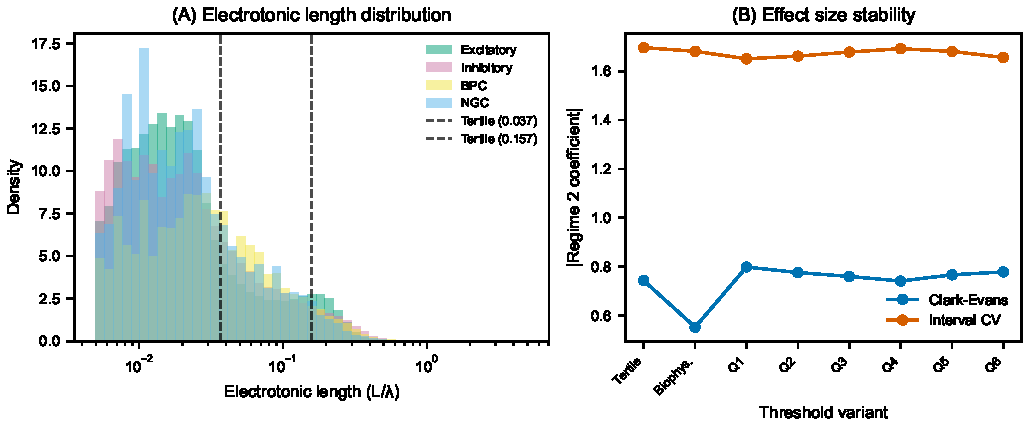
\includegraphics[width=0.95\textwidth]{../figures/fig1_electrotonic_sensitivity.pdf}
\caption{\textbf{Electrotonic length distribution and sensitivity analysis.} (A) Distribution of branch electrotonic lengths ($L/\lambda$) across 136,414 branches from 2,138 neurons. Vertical dashed lines indicate tertile thresholds. (B) Sensitivity of the regime 2 coefficient to threshold choice across eight discretization schemes for three spatial metrics. All 24 models converge, with Clark-Evans coefficients ranging from 0.55 to 0.80.}
\label{fig:electrotonic}
\end{figure}

\begin{figure}[H]
\centering
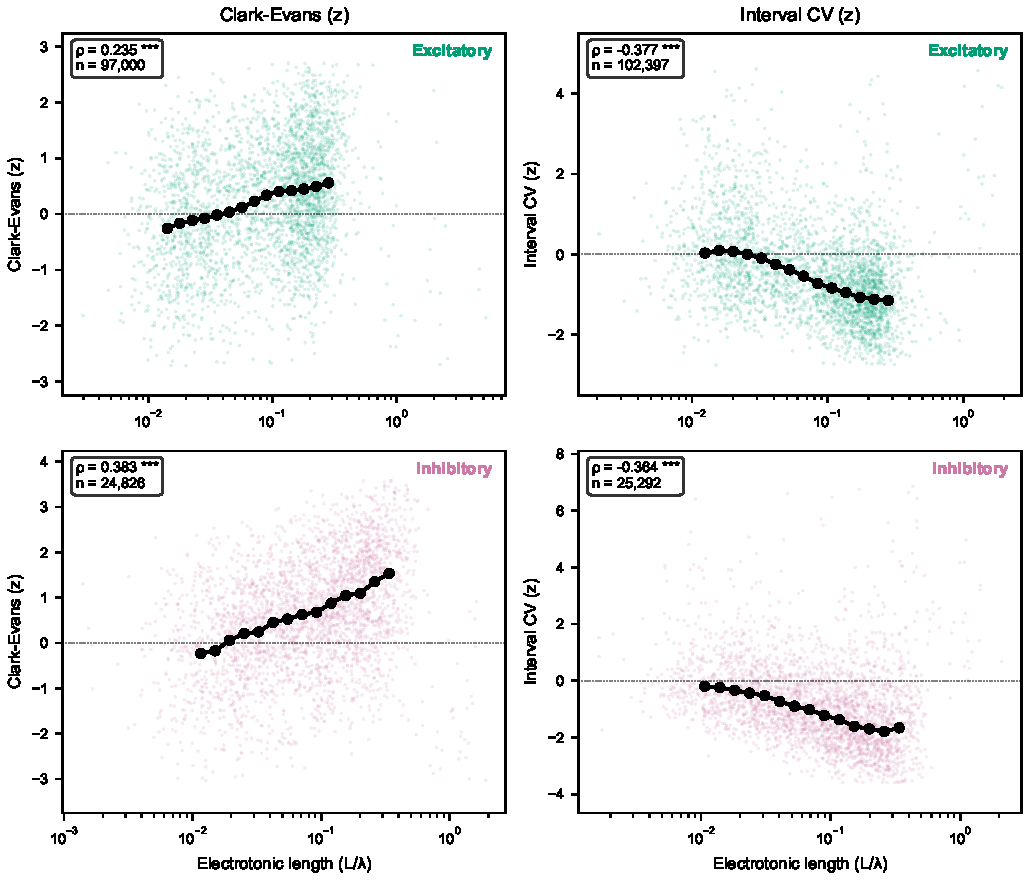
\includegraphics[width=0.95\textwidth]{../figures/fig2_continuous_scatterplots.pdf}
\caption{\textbf{Synaptic spatial organization tracks with continuous electrotonic length.} Scatter plots of $L/\lambda$ vs.\ spatial metric $z$-scores for excitatory (top) and inhibitory (bottom) neurons, with binned medians (orange) computed in the 5th--95th percentile core ($\geq 20$ points per bin). Left: Clark-Evans $z$. Right: Interval CV $z$. Inhibitory neurons show steep, monotonic trends ($\beta = 7.65$, $p < 10^{-77}$ and $\beta = -17.5$, $p < 10^{-90}$, respectively). Excitatory neurons show significant but weaker continuous relationships.}
\label{fig:continuous}
\end{figure}

\begin{figure}[H]
\centering
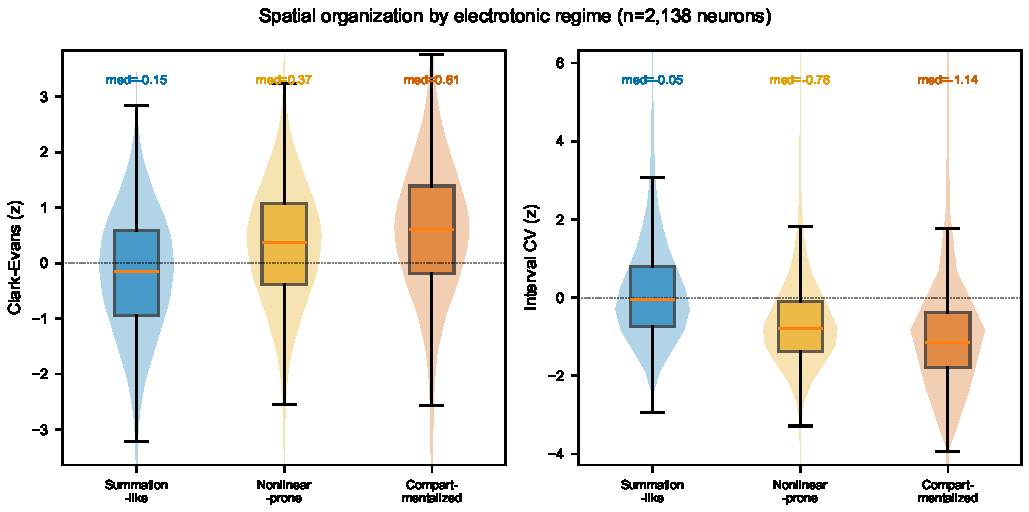
\includegraphics[width=0.95\textwidth]{../figures/fig3_regime_violin.pdf}
\caption{\textbf{Discretized regime analysis.} Violin plots of spatial metric $z$-scores stratified by electrotonic regime (0: compact, 1: intermediate, 2: compartmentalized) for 2,138 neurons. Clark-Evans $z$ and Interval CV $z$ show monotonic dose-response. Pairwise compactness $z$ shows non-monotonic behavior with a regime 1 reversal. All regime 2 vs.\ regime 0 comparisons: $p < 10^{-300}$.}
\label{fig:regime}
\end{figure}

\begin{figure}[H]
\centering
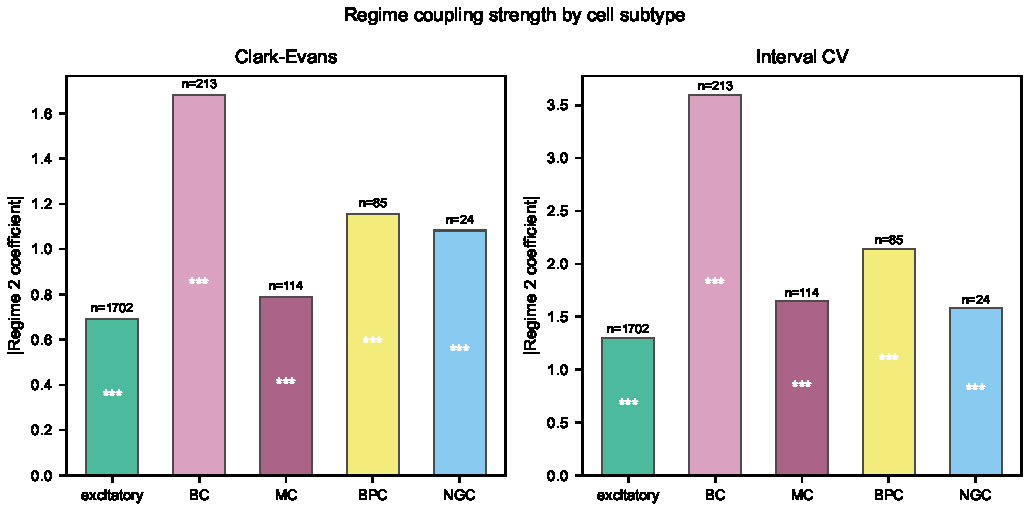
\includegraphics[width=0.95\textwidth]{../figures/fig4_subtype_effects.pdf}
\caption{\textbf{Cell-type-specific coupling strength.} Clark-Evans regime 2 coefficients and Cohen's $d$ effect sizes for 11 cell types. All four inhibitory subtypes (blue shades) show stronger coupling than the excitatory aggregate (orange). Basket cells are the strongest ($d = 1.15$); Martinotti cells are the weakest inhibitory subtype ($d = 0.64$) but still exceed the excitatory mean ($d = 0.60$). Error bars: 95\% confidence intervals from mixed-effects models.}
\label{fig:subtype}
\end{figure}

\begin{figure}[H]
\centering
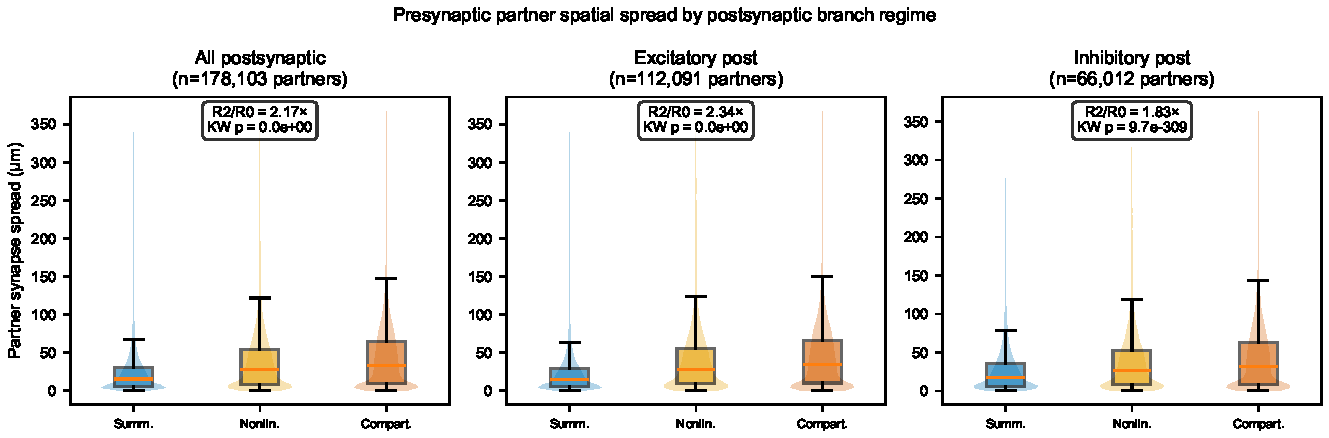
\includegraphics[width=0.85\textwidth]{../figures/fig5_partner_compactness.pdf}
\caption{\textbf{Partner spatial spread by electrotonic regime.} Mean 3D pairwise distance of synapses from individual presynaptic partners ($k \geq 3$ synapses), classified by the dominant regime of innervated branches. Partners on regime 2 branches spread their synapses 2.17-fold wider than partners on regime 0 branches ($n = 178{,}103$ partners).}
\label{fig:partner}
\end{figure}


% ============================================================
% SUPPLEMENTARY
% ============================================================
\clearpage
\section*{Supplementary Figures}

\begin{figure}[H]
\centering
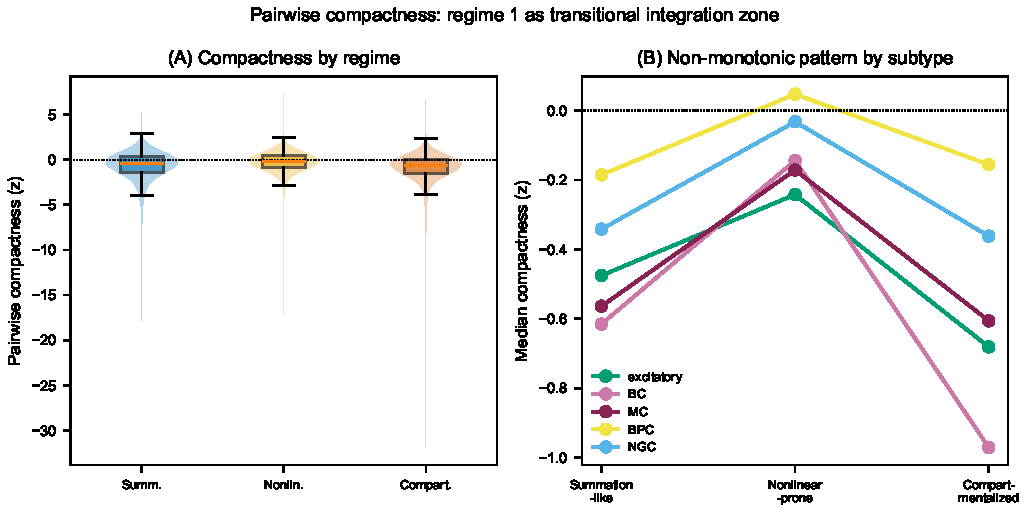
\includegraphics[width=0.95\textwidth]{../figures/figS1_compactness_nonmonotonic.pdf}
\caption{\textbf{Figure S1. Pairwise compactness non-monotonicity across cell types.} Dose-response plots of median pairwise compactness $z$-score by electrotonic regime, stratified by cell type. The regime 1 reversal (dip below regime 0 and regime 2) is consistent across excitatory and all four inhibitory subtypes, ruling out a subtype-specific artifact. MC compactness coupling is not significant in the continuous analysis (Spearman $p = 0.15$), consistent with the weakest overall coupling among inhibitory subtypes.}
\label{fig:compactness_nonmono}
\end{figure}

\begin{figure}[H]
\centering
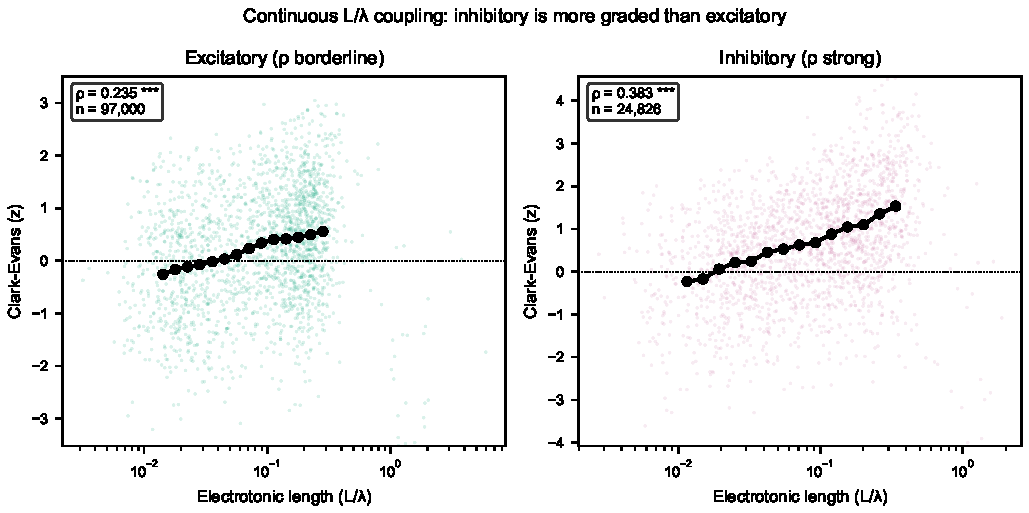
\includegraphics[width=0.95\textwidth]{../figures/figS2_exc_inh_continuous.pdf}
\caption{\textbf{Figure S2. Excitatory vs.\ inhibitory continuous coupling.} Direct comparison of $L/\lambda$ vs.\ spatial metric $z$-scores between excitatory and inhibitory neurons. Inhibitory neurons show steeper slopes across all metrics. For pairwise compactness, the excitatory continuous relationship is null ($p = 0.67$) while the inhibitory relationship is strong ($p < 10^{-117}$), demonstrating that the metric-specific divergence is cell-type-dependent.}
\label{fig:exc_inh_continuous}
\end{figure}

\bibliographystyle{apalike}
\bibliography{references}

\end{document}
